\section{Circunferencia de los nueve puntos y Recta de Simson}

\begin{sol}
	
	\begin{figure}[h!]
		\centering
		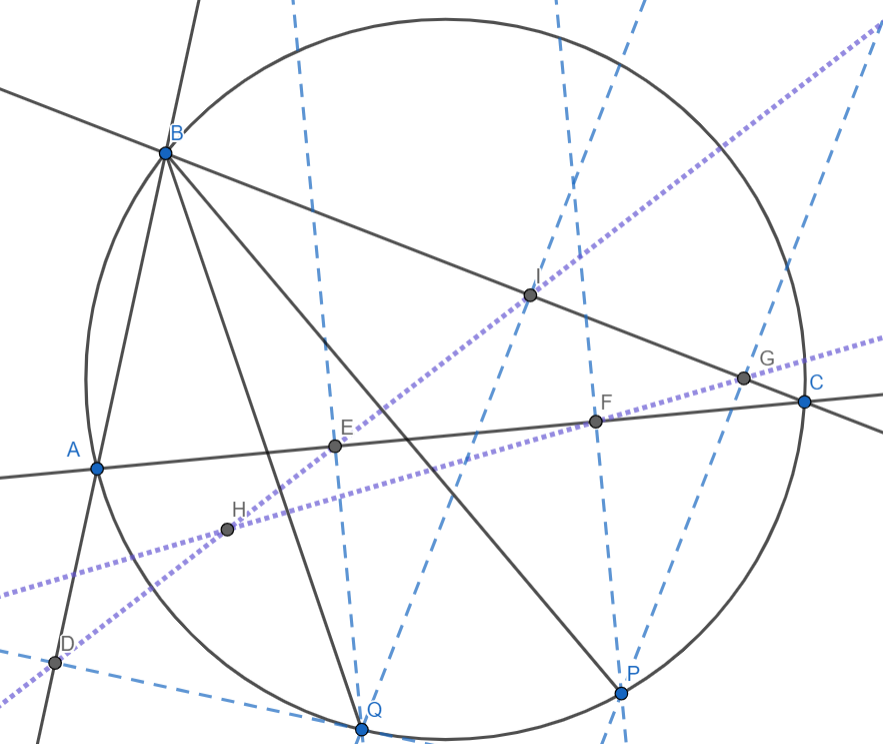
\includegraphics[scale=0.4]{Imgs/JT5.png}
	\end{figure}
	Llame $\omega_{1} = \angle QBP, \omega_{2} = \angle ABQ, \omega_{3} = \angle BCA$. Como el cuadril\'atero $DBIQ$ es c\'iclico, tenemos que $\angle DIQ = \omega_{2}$. Ademas, observemos que si llamamos de $X = FH \cap IQ$, $Y = QI \cap FP$, entonces $\angle IXF = \angle HFP - \angle QYF$. Adem\'as, como $YIFC$ es c\'iclico $\implies \angle IXF = \angle ICF = \omega_{3}$. Sigue que $\angle IXF = \angle GCP - \omega_{3}$ ($FGCP$ es c\'iclico). Pero $\angle GCP = \omega_{3} + \omega_{1} + \omega_{2}$. Luego, $\angle IXF = \omega_{1} + \omega_{2}$. Finalmente, $\angle FHI = \angle IXF - \angle HIQ = \omega_{1}$. 
\end{sol}

\begin{sol}
	Los siguientes cuadril\'ateros son c\'iclicos: $RQNB$ $(1)$, $QHWN$  $(2)$, $WSCN$ $(3)$, $APHM$ $(4)$, $BPMC$ $(5)$, donde $H$ es el ortocentro del tri\'angulo original. Entonces, tenemos que $(1) \implies \angle RQB = \angle RNB = \angle PCB$ (pues $PC \parallel RN$) $(5) \implies \angle PCB = \angle PMB$. La primera con la \'ultima igualdad de la cadena implican que $PM \parallel RQ$. $(2) \implies \angle HQW = \angle HNW = \angle PAH$ ( debido a que $AP \parallel WN$) $(4) \implies \angle PAH = \angle PMH$. De nuevo, la cadena implica que $QW \parallel PM$. An\'alogamente, $WS \parallel PM$, y se concluye la primera parte.
	
	Para la segunda parte, llame $Q' \in PM$ tal que $Q'Q \parallel AB$, Lo mismo con $W' \in PM$, tal que $W'W \parallel AC$. El problema se reduce a demostrar que $Q' = W'$. En efecto, observemos que 
	\begin{align}
	\frac{MQ'}{Q'P} = \frac{MQ}{QB} = \frac{CN}{NB} = \frac{CW}{WP} = \frac{PW'}{W'P}
	\end{align}
	Puesto que $QQ' \parallel AB$, $WN \parallel AC$, $WN \parallel AB$, $WW' \parallel AC$, respectivamente. De la primera y \'ultima igualdad de la cadena, sigue que $W' = Q'$, como dese\'abamos. 
\end{sol}

\begin{sol}
	Observe que las rectas $PQ$, $RS$ y $AB$ concurren en un punto que se llamar\'a $F$. En efecto, $PQ$ es la recta de Simson de $Y$ con respecto a $\triangle AXB$ y $RS$ con respecto al tri\'angulo $\triangle AZB$. Luego, ambas rectas concurren en el tercer punto de la recta de Simson, es decir, la base de la altura de $Y$ con respecto a $AB$ (es decir, $YF \perp AB$). Observemos que $\angle YFB = 90^{\circ} = \angle YSB$. Es decir, el cuadril\'atero $YSBF$ es c\'iclico y tambi\'en  $YPAF$, de manera an\'aloga. En particular, $\angle PAY = \angle PFY$, y $\angle SBY = \angle YFS$. La siguiente cadena de desigualdades termina el ejercicio: $\angle PFS = \angle YFP + \angle YFS = \angle SBY + \angle YAP = \angle SBY + \angle XBY = \angle ZBX = \frac{\angle XOZ}{2}$. Como quer\'iamos. 
	
	\begin{figure} [h!]
		\centering
		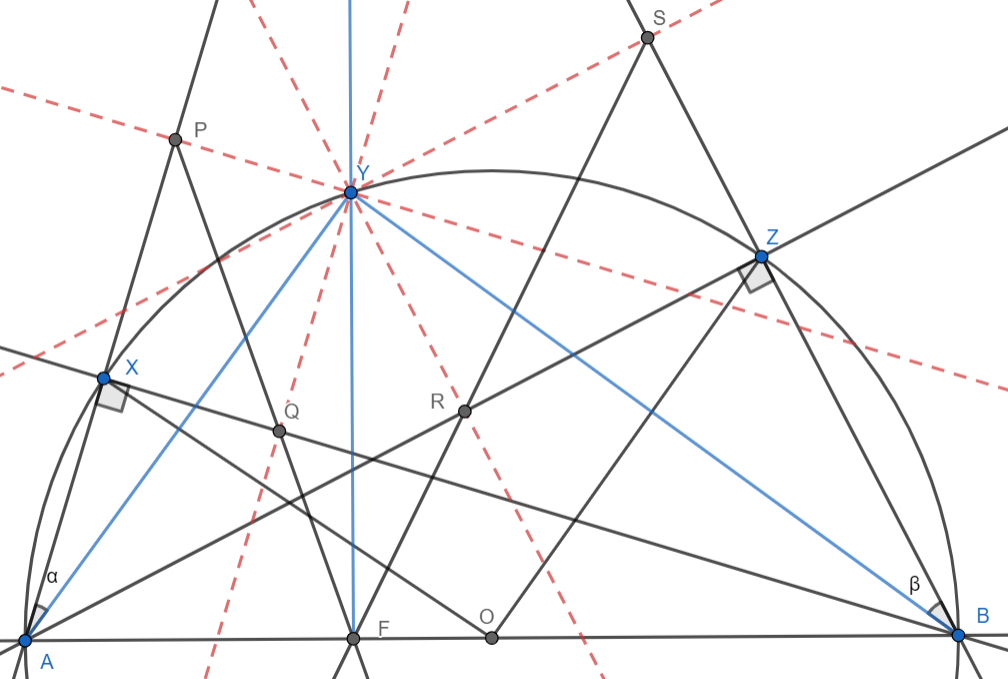
\includegraphics[scale=0.4]{Imgs/JT6.png}
	\end{figure}

	
\end{sol}




\begin{sol}
	Observe que si $Q_{1}$ es el circuncentro de $\triangle PBC$, $Q_{2}$ el de $\triangle PAC$ y $Q_{3}$ el de $\triangle PAB$, entonces $Q_{2}Q_{1} \perp PC $, $Q_{2}Q_{3} \perp PA$. Basta entonces con demostrar que $\angle Q_{3}PQ_{1} = \angle APC$.
	
	\textbf{Lemma}: En un tri\'angulo $\triangle ABC$ con circuncentro $O$, se cumple que $\angle OAC + \angle ABC = 90^{\circ}$ (Admitiendo angulos negativos si el circuncentro se encuentra fuera del tri\'angulo!).
	
	\textit{Prueba}: Hecho conocido.
	
	Aplicamos el hecho en los tri\'angulos $\triangle APB $ y $\triangle PBC$. Obtenemos entonces que $\angle Q_{3}PA + \angle PBA = 90^{\circ}$ y $\angle Q_{1}PC + \angle PBC = 90^{\circ}$. Sumando ambos t\'erminos, obtenemos que $\angle Q_{3}PA + \angle PBA  + \angle Q_{1}PC + \angle PBC = 180^{\circ} \implies \angle Q_{3}PA = -\angle Q_{1}PC$. Puede parecer raro, pero lo \'unico que nos dice es que ambos \'angulos tienen la misma magnitud, solo que uno de los puntos (y solo uno de ellos!) se encuentra fuera del tri\'angulo $\triangle ABC$. La igualdad $\angle Q_{3}PQ_{1} = \angle APC + \angle Q_{3}PA + \angle Q_{1}PC$ esclarece un poco las cosas.
	
\end{sol}

\begin{sol}
	

		Es un hecho conocido que el circuncentro y el ortocentro de un tri\'angulo son conjugados isogonales, asi que podemos asumir que $BI$ y $CI$ son bisectrices de $\angle OBH$ y $\angle OCH$ (no hace falta usar ese hecho, es la forma mas corta que conozco, eso es todo), respectivamente. Usando el teorema de la bisectriz en ambos tri\'angulos obtenemos que
		\begin{align}
		\frac{BO}{BH} = \frac{OI}{IH} = \frac{CO}{CH} \implies BH = CH
		\end{align}
		
		Debido a que $CO = BO$. Pero entonces $I$ pertenece a la mediatriz de $BC$, y por lo tanto $\angle ABC = \angle ACB\square$.

\end{sol}

\begin{sol}
	Sea $S$ la recta de Simson de $P$ con respecto a $\triangle ABC$. Sea $\Omega$ el circunc\'irculo de $\triangle ABC$. Definamos los siguientes puntos: $F = AH \cap BC$ , $ E = AH \cap \Omega$ , $ Z = S \cap BC$ , $ Y = S \cap AB$ , $ Q = PZ \cap \Omega$ , $ D = PE \cap BC$ , $ R = HD \cap PQ$.
	
	\textbf{Lemma 1}: $HF = FE$. 
	
	\textit{Prueba}: Simplemente observe que los tri\'angulos $\triangle BFC$ y $\triangle BCE$ son congruentes y comparten un lado en com\'un $\square$.
	
	\textbf{Lemma 2} $S \parallel AQ \parallel HR$ 
	
	\textit{Prueba}: Observe que $BYZP$ es c\'iclico, por lo tanto $\angle AYM = \angle BPQ = \angle QAB$, debido a que $QBPA$ es c\'iclico. Sigue que $QA \parallel S$. Ahora, veamos que como $QP \parallel AE$, el trapecio $QPEA$ es is\'oceles. EL hecho de que $QP \parallel ZD$ y $HF = FE$ implican que $RZ =ZP$. Por lo tanto $RD \parallel QA$ $\square$.
	
	Por la proposici\'on anterior (Teorema de Thales), $1= \frac{PZ}{RZ} = \frac{PM}{HM}$, y el resultado sigue.
\end{sol}

\begin{sol}
	
	Sea $H_{B}$ el ortocentro de $\triangle ACD$, y $H_{D}$ el ortocentro de $\triangle BAC$. Lo que se va a demostrar es que, usando el ejercicio anterior, todos los puntos medios de los segmentos $P-$ortocentro coinciden. En este caso, los segmentos son $BH_{B}$ y $DH_{D}$. Para tal efecto, veamos que como $H_{D}B \parallel H_{B}D$, es suficiente probar que el cuadril\'atero formado por \'estos cuatro puntos es un paralelogramo, y por lo tanto el punto medio de las diagonales es el mismo. La siguiente cadena de igualdades muestra tal hecho: 
	
	\begin{align}
	\angle BDH_{D} &= \angle ADC - \angle ADB - \angle H_{B}DC = \angle ADC - \angle BCA - \angle H_{B}AC \\
	\angle BH_{D}H_{B} &= \angle AH_{D}C - \angle AH_{D}B - \angle H_{B}H_{D}C = \angle AH_{D}C -\angle BCA - \angle H_{B}AC
	\end{align}
	 Donde usamos que $ABCD$ es c\'iclico, dos veces. Queda entonces demostrar que $\angle ADC = \angle AH_{D}C$. Pero eso es simple, una vez que $\angle ABC + \angle AH_{D}C = 180^{\circ} = \angle ABC + \angle ADC$. El resultado sigue
	 
	 \begin{figure}[h!]
	 	\centering
	 	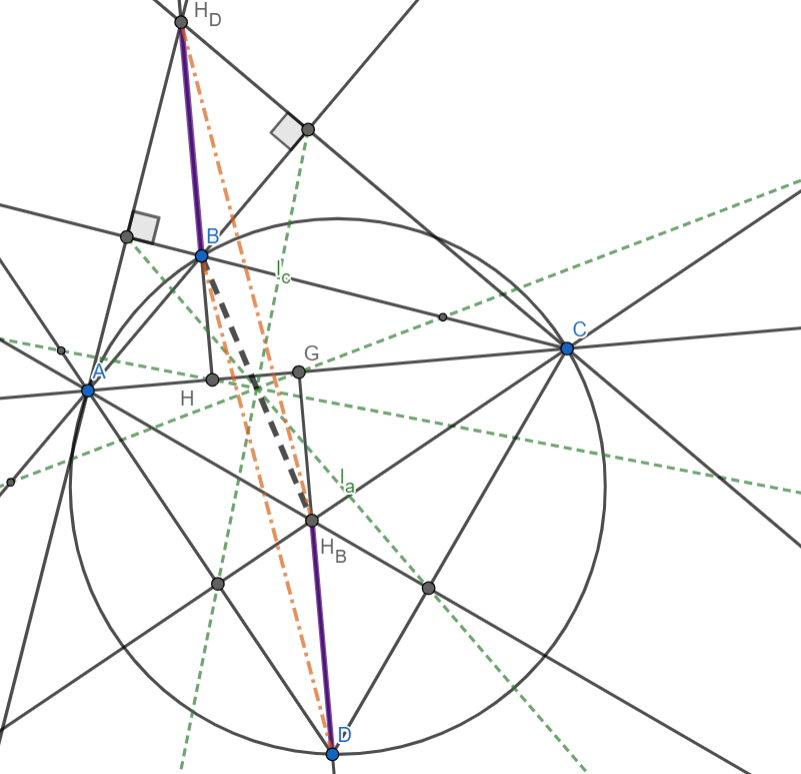
\includegraphics[scale=0.5]{Imgs/JT7.png}
	 \end{figure}
	 
\end{sol}

\begin{sol}
	Soluci\'on pendiente :(
\end{sol}

\begin{sol}
	Sea $H, F, G$ las bases de las perpendiculares de $P$ trazadas con respecto a $BC$, $AB$ y $AC$ respectivamente. Sea $M = AQ \cap FH$. Observemos que $PFBH$ es c\'iclico, por lo tanto $\angle PBF = \angle FHP$. Adem\'as, los puntos $P, A, Q, B$ son conc\'iclicos, por lo tanto $\angle PBF = \angle PQA$. Sique que $\angle FHP = \angle PQM \implies M, Q, H, P $ son conc\'iclicos $\implies \angle HDE = \angle HMQ = 90^{\circ}\square$.
\end{sol}

\begin{sol}
	\begin{enumerate}[a.]
		\item Observe que todos los tri\'angulos, $\triangle ABC,\triangle HBC,\triangle AHC,\triangle ABH$ poseen algunos  de los puntos pertenecientes a la circunferencia de los nueve puntos de $\triangle ABC$. Por ejemplo, el tri\'angulo $\triangle AHC$ tiene las mismas alturas que $\triangle ABC$. Como una circunferencia est\'a determinada por tres puntos solamente, obtenemos que todas ellas son la misma. 
		\item Simplemente observe que la recta de Euler siempre pasa por el centro de la circunferencia de los nueve puntos. Como este centro es el mismo para todos los tri\'angulos, el resultado sigue.
	\end{enumerate}
\end{sol}